\newpage
\section[Day 2: Fields]{Day 2: Fields}





\subsection{Greatest Upper Bound Property}

{ \color{red} Theorem 2.1.1: Least Upper Bound + Lower Bound implies Greatest Upper Bound }
	\begin{adjustbox}{minipage=14cm, right}
		Let S be a ordered set with the least upper bound property.

		Let non-empty B $\subset$ S be bounded below.

		Let L be the set of all lower bounds of B.

		Then $\alpha$ = sup(L) exists in S.
	\end{adjustbox}

{ \color{magenta} \underline{Proof} }

	L is non-empty since B is bounded from below.

	Thus, by the least upper bound property of S, $\alpha$ = sup(L) exists in S.

	We claim that $\alpha$ = inf(B).

	If $\gamma < \alpha$, then $\gamma$ is not an upper bound for L so y $\not \in$ B.

	Thus, for every x $\in$ B, $\alpha \leq$ x.

	If $\gamma \geq \alpha$, then $\gamma$ is an upper bound of L so $\gamma \in$ B.
	Thus, inf(B) = $\alpha$.

\begin{figure}[h]
	\centering
	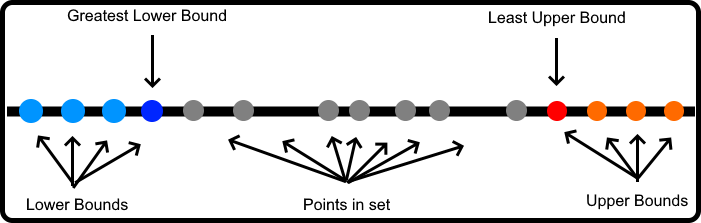
\includegraphics[scale=0.45]{Images/2.1.png}
	\caption{Infimum, Supremum, \& Bounds}
\end{figure}





\subsection{Fields}

Addition Axioms
	\begin{itemize}[leftmargin=1cm, itemsep=0.4em]
		\item If x,y $\in$ F, then x+y $\in$ F
	
		\item x+y = y+x for all x,y $\in$ F
	
		\item (x+y)+z = x+(y+z) for all x,y,z $\in$ F
	
		\item There exists 0 $\in$ F such that 0+x = x for all x $\in$ F
	
		\item For every x $\in$ F, there is -x $\in$ F where x+(-x) = 0
	\end{itemize}

Multiplicative xioms
	\begin{itemize}[leftmargin=1cm, itemsep=0.4em]
		\item If x,y $\in$ F, then xy $\in$ F
	
		\item yx = xy for all x,y $\in$ F
	
		\item (xy)z = x(yx) for all x,y,z $\in$ F
	
		\item There exists 1 $\not =$ 0 $\in$ F such that 1x = x for all x $\in$ F
	
		\item If x $\not =$ 0 $\in$ F, there is $\frac{1}{x}$ $\in$ F where x($\frac{1}{x}$) = 1
	\end{itemize}

Distributive Law

	\qquad x(y+z) = xy + xz hold for all x,y,z $\in$ F. \\

{ \color{blue} Propositions 2.2.1 }
	\begin{enumerate}[label=(\alph*), leftmargin=2cm, itemsep=0.4em]
		\item If x+y = x+z, then y = z

			{ \color{magenta} \underline{Proof}  }
		
				y = 0+y = (-x)+x+y = (-x)+x+z = 0+z = z
			
		\newpage
	
		\item If x+y = x, then y = 0

			{ \color{magenta} \underline{Proof} }

				From (a), let z = 0.
	
		\item If x+y = 0, then y = -x
	
			{ \color{magenta} \underline{Proof} }

				From (a), let z = -x.
	
		\item -(-x) = x

			{ \color{magenta} \underline{Proof} }

				From (c), let x = -x and y = x.
	
		\item If x $\not =$ 0 and xy = xz, then y = z

			{ \color{magenta} \underline{Proof} } 
		
				y = 1y = $\frac{1}{x}$xy = $\frac{1}{x}$xz = 1z = z 
	
		\item If x $\not =$ 0 and xy = x, then y = 1

			{ \color{magenta} \underline{Proof} } 
		
				From (e), let z = 1.
	
		\item If x $\not =$ 0 and xy = 1, then y = $\frac{1}{x}$

			{ \color{magenta} \underline{Proof} } 
		
				From (e), let z = $\frac{1}{x}$.
	
		\item If x $\not =$ 0, then $\frac{1}{1/x}$ = x

			{ \color{magenta} \underline{Proof} } 
		
				From (g), let x = $\frac{1}{x}$ and y = x.
	
		\item 0x = 0

			{ \color{magenta} \underline{Proof} } 
		
				Since 0x + 0x = (0+0)x = 0x, then 0x = 0.
	
		\item If x,y $\not =$ 0, then xy $\not =$ 0

			{ \color{magenta} \underline{Proof} } 
		
				Suppose xy = 0, then $\frac{1}{y}\frac{1}{x}$xy
				= $\frac{1}{y}$1y = $\frac{1}{y}$y = 1.

				xy = 0 = 1 is a contradiction.
	
		\item (-x)y = -(xy) = x(-y)

			{ \color{magenta} \underline{Proof} } 
		
				xy + (-x)y = (x+(-x))y = 0y = 0.

				Then by part (c), (-x)y = -(xy).

				Similarly, xy + x(-y) = x(y+(-y)) = x0 = 0.
	
				Then by part (c), x(-y) = -(xy).

		\item (-x)(-y) = xy

			{ \color{magenta} \underline{Proof} } 
		
				By part (k), then (-x)(-y) = -[x(-y)] = -[-(xy)].

				By part (d), -[-(xy)] = xy.
	\end{enumerate}





\subsection{Ordered Fields}

	\qquad An ordered field F is a field F which is also an ordered set for all x,y,z $\in$ F.

	\begin{itemize}[leftmargin=2cm, itemsep=0.4em]
		\item If y $<$ z, then y+x $<$ z+x
	
		\item If x,y $>$ 0, then xy $>$ 0
	\end{itemize}

\newpage

{ \color{blue} Definition 2.3.1: $ \mathbb{Q} $ and $ \mathbb{R} $ are ordered fields } 

	\qquad $ \mathbb{Q} $ , $ \mathbb{R} $ are ordered fields,
	but $ \mathbb{C} $ is not an ordered field since i$^2$ = -1 $\not >$ 1. \\

{ \color{blue} Propositions 2.3.2} 

	\qquad Let F be an ordered field. For all x,y,z $\in$ F.
	\begin{enumerate}[label=(\alph*), leftmargin=2cm, itemsep=0.4em]
		\item If x $>$ 0, -x $<$ 0 and vice versa
	
			{ \color{magenta} \underline{Proof} } 
	
				-x = (-x) + 0 $<$ (-x) + x = 0

		\item If x $>$ 0 and y $<$ z, then xy $<$ xz
	
			{ \color{magenta} \underline{Proof} } 
		
				Since z-y $>$ 0, then 0 $<$ x(z-y) = xz - xy

		\item If x $ < $ 0 and y $ < $ z, then xy $ > $ xz

			{ \color{magenta} \underline{Proof} } 
		
				Since -x $>$ 0 and z-y $>$ 0, then 0 $<$ -x(z-y) = xy - xz
	
		\item If x $\neq$ 0, $x^2 > $ 0

			{ \color{magenta} \underline{Proof} } 
		
				If x $>$ 0, then x$^\text{2}$ = x $\cdot$ x $>$ 0

				If x $<$ 0, then x$^\text{2}$ = (-x) $\cdot$ (-x) $>$ 0
	
		\item If 0 $< x < y$, then 0 $< 1/y < 1/x$

			{ \color{magenta} \underline{Proof} } 
		
				Since ($\frac{1}{\text{y}}$)y = 1 $>$ 0, then ($\frac{1}{\text{y}}$) $>$ 0

				Since x $<$ y, then $\frac{1}{\text{y}}$
				= ($\frac{1}{\text{y}}$)($\frac{1}{\text{x}}$)x
				$<$ ($\frac{1}{\text{y}}$)($\frac{1}{\text{x}}$)y = $\frac{1}{\text{x}}$ \\
	\end{enumerate}

{\color{red} Theorem 2.3.3: $\mathbb{R}$ is a ordered field with $<$ }

	\qquad There exists a unique ordered field $ \mathbb{R} $ with the least upper bound property.

	\qquad Also, $ \mathbb{Q} $  $\subset$ $ \mathbb{R} $ so $\mathbb{Q}$ is also an ordered field. \\

{\color{red} Theorem 2.3.4}

	For all x,y $\in$ $ \mathbb{R} $:
	\begin{itemize}[leftmargin=1cm, itemsep=0.4em]
		\item {\color{lblue} Archimedean Property}:
			If x $>$ 0, there is n $\in$ $ \mathbb{Z} $ such that nx $>$ y.
	
			{ \color{magenta} \underline{Proof} }

				Fix x $>$ 0. Suppose there is a y such that the property fails.

				Let A = \{ nx: n = 1, 2, 3, ... \}.

				Then, A is nonempty and bounded from above by y.

				Then by the least upper bound property by $ \mathbb{R} $,
				$\alpha$ = sup(A) exists in $ \mathbb{R} $ .

				Since x $>$ 0, then -x $<$ 0 so $\alpha - x < \alpha-0 = \alpha$.

				So $\alpha-x$ is not an upper bound of A.

				So there is a mx $\in$ A such that mx $> \alpha-x$.

				Then $\alpha <$ (m+1)x, but (m+1)x $\in$ A
				contradicting $\alpha$ is an upper bound for A.

		\item {\color{lblue} $ \mathbb{Q} $  is dense in $ \mathbb{R} $}:
			If x $<$ y, there is a p $\in$ $ \mathbb{Q} $ such that x $<$ p $<$ y.

			{ \color{magenta} \underline{Proof} }

				Since x $<$ y, then y-x $>$ 0. Then by the Archimedean Property,
				there exists a n $\in$ Z such that n(y-x) $>$ 1. Thus, ny $>$ nx+1 $>$ nx

				By the well-ordering principle, there is a smallest m $\in \mathbb{Z_+} $
				such that m $>$ nx.

				Then, m $>$ nx $\geq$ m-1 so nx+1 $\geq$ m $>$ nx.

				Since ny $>$ nx+1 $\geq$ m $>$ nx, then y $>$ m/n $>$ x.
\end{itemize}
